\documentclass[11pt]{article}
\usepackage[preprint]{acl}
\usepackage{times}
\usepackage{latexsym}
\usepackage[T1]{fontenc}
\usepackage[utf8]{inputenc}
\usepackage{microtype}
\usepackage{inconsolata}
\usepackage{graphicx}
\usepackage{amsmath}

\setlength\titlebox{5.0cm}

\title{Retrieval-Based Scientific Claim Verification with SciFact}

\author{Jiapei Liao \\
  Boston University \\
  \texttt{jiapei03@bu.edu}
  \And
  Yuxiang Liu \\
  Boston University \\
  \texttt{mat1900@bu.edu}}

\begin{document}
\maketitle

\begin{abstract}
We study scientific claim verification on SciFact, where a system must retrieve evidence-bearing biomedical abstracts and predict whether the evidence \textsc{Supports}, \textsc{Refutes}, or provides \textsc{NoInfo} for a claim. We build a two-stage pipeline with abstract retrieval followed by document-level stance verification, and compare lexical baselines against dense retrieval and pretrained biomedical encoders. Dense MPNet retrieval improves evidence retrieval over TF--IDF, raising Recall@5 from 0.803 to 0.872 and MRR from 0.657 to 0.743. For verification, fine-tuned \textsc{SciBERT} improves oracle macro-F1 from 0.359 for logistic regression to 0.676. In the full pipeline, Dense+\textsc{SciBERT} reaches JointHit@5 of 0.521. We further add error analysis, a sentence-level evidence-selection experiment, and a \textsc{PubMedBERT} verifier. The strongest final system, Dense+\textsc{PubMedBERT}, reaches JointHit@5 of 0.564. Our analysis shows that retrieval is no longer the dominant bottleneck: at top-5, only 12.8\% of evidence-bearing claims are retrieval misses, while 35.1\% fail because a retrieved gold abstract receives the wrong stance label.
\end{abstract}

\section{Introduction}
Scientific claim verification asks whether a natural-language scientific claim is supported or contradicted by evidence in the literature. This is more difficult than ordinary document retrieval because lexical relevance is not enough: an abstract can mention the same entities as a claim while failing to verify it, and a true evidence abstract may use different wording from the claim. We use SciFact, a closed-corpus benchmark with 1,409 expert-written claims and 5,183 biomedical abstracts, to study this problem in a realistic but manageable setting \citep{wadden2020fact}.

Our project focuses on abstract retrieval and abstract-level stance classification. Given a claim $c$ and a corpus $\mathcal{D}$, the retriever returns the top-$k$ candidate abstracts,
\begin{equation}
R_k(c) = \operatorname{TopK}_{a \in \mathcal{D}}\; \mathrm{sim}(g(c), g(a)).
\end{equation}
For each retrieved claim--abstract pair $(c,a)$, a verifier predicts
\begin{equation}
\hat{y}=f_{\theta}(c,a), \qquad
\hat{y}\in\{\textsc{Supports},\textsc{Refutes},\textsc{NoInfo}\}.
\end{equation}
The full system succeeds only when it retrieves a gold evidence abstract and assigns the correct stance label.

The midway version of the project implemented the core two-stage pipeline and showed that dense retrieval plus a fine-tuned \textsc{SciBERT} verifier strongly outperformed a lexical TF--IDF plus logistic-regression baseline. In the final stage, we extend that work in three directions: detailed error analysis, a sentence-level evidence-selection experiment, and a stronger biomedical verifier based on \textsc{PubMedBERT} \citep{gu2021domain}. These additions let us ask not only which system performs best, but also where the remaining failures come from.

\section{Methods}
\subsection{Dataset and Pair Construction}
We use the official SciFact train and development splits \citep{wadden2020fact}. The train split contains 809 claims, the development split contains 300 claims, and the corpus contains 5,183 abstracts. Because the public test labels are not available, all reported quantitative results are on the development set.

To train verifiers, we construct document-level claim--abstract pairs. Each annotated evidence document becomes a positive pair labeled \textsc{Supports} or \textsc{Refutes}. For each claim, we also add four \textsc{NoInfo} negative pairs. These negatives are sampled first from cited but non-evidence documents, then from TF--IDF hard negatives, and finally from random corpus documents when needed. This produces 3,800 training pairs and 1,409 development pairs. The development pair labels are imbalanced: 1,200 \textsc{NoInfo}, 138 \textsc{Supports}, and 71 \textsc{Refutes} examples, so macro-F1 is a more informative verifier metric than accuracy alone.

\subsection{Retrieval Models}
Our lexical retriever is a TF--IDF model over each document's title and abstract, using unigram and bigram features. Our dense retriever uses \texttt{sentence-transformers/all-mpnet-base-v2}, which encodes claims and abstracts into a shared embedding space and ranks documents by cosine similarity \citep{reimers2019sentence,song2020mpnet}. The dense retriever is used as a fixed pretrained encoder rather than being fine-tuned on SciFact.

\subsection{Verification Models}
The lexical verifier is multinomial logistic regression over TF--IDF features of the concatenated claim and abstract. We compare it with two transformer verifiers. The first is \texttt{allenai/scibert\_scivocab\_uncased}, a domain-specific encoder pretrained on scientific text \citep{beltagy2019scibert}. The second is \texttt{microsoft/BiomedNLP-PubMedBERT-base-uncased-abstract-fulltext}, which is pretrained from scratch on biomedical literature \citep{gu2021domain}. Both transformer verifiers are fine-tuned for three-way classification with class-weighted cross-entropy, mixed-precision GPU training, learning rate $2\times10^{-5}$, batch size 16, maximum sequence length 256, and checkpoint selection by internal development macro-F1.

\subsection{Sentence-Level Evidence Selection}
The midway system treated entire abstracts as evidence units. We test whether a targeted evidence-selection stage can improve verification. We implement an unsupervised TF--IDF sentence selector: for each claim--abstract pair, it ranks sentences in the abstract by cosine similarity to the claim and keeps the top two sentences, preserving their original abstract order. We evaluate this selector directly against gold SciFact rationale sentence annotations, and we also train a \textsc{SciBERT} verifier on the selected sentence text instead of full abstracts.

\subsection{Evaluation Metrics}
For retrieval, we report Recall@$k$ and mean reciprocal rank (MRR) over evidence-bearing development claims. For oracle verification, we evaluate verifiers on gold and negative claim--document pairs using accuracy, macro-F1, and per-class F1. For the full pipeline, we report JointHit@$k$: a claim is counted as correct if at least one gold evidence abstract appears in the top-$k$ retrieved list and receives the correct stance label. For sentence selection, we report rationale Hit@$k$ and rationale Coverage@$k$ over gold claim--document evidence pairs.

\section{Results}
\subsection{Retrieval}
Dense retrieval clearly improves over the TF--IDF retriever (Table~\ref{tab:retrieval}). The gain is consistent across all cutoffs: Recall@5 increases from 0.803 to 0.872, Recall@10 from 0.856 to 0.931, and MRR from 0.657 to 0.743. This confirms that semantic matching helps recover evidence abstracts that are not captured by lexical overlap alone.

\begin{table}[t]
\centering
\small
\begin{tabular}{lcccc}
\hline
\textbf{Retriever} & \textbf{R@3} & \textbf{R@5} & \textbf{R@10} & \textbf{MRR} \\
\hline
TF--IDF & 0.761 & 0.803 & 0.856 & 0.657 \\
Dense MPNet & \textbf{0.798} & \textbf{0.872} & \textbf{0.931} & \textbf{0.743} \\
\hline
\end{tabular}
\caption{Retrieval performance on evidence-bearing SciFact development claims.}
\label{tab:retrieval}
\end{table}

\subsection{Oracle Verification}
Table~\ref{tab:oracle} shows that transformer verifiers substantially outperform the lexical verifier. Logistic regression achieves high accuracy because most development pairs are \textsc{NoInfo}, but its macro-F1 is only 0.359 and it performs very poorly on \textsc{Supports} and \textsc{Refutes}. \textsc{SciBERT} improves macro-F1 to 0.676, with much stronger positive-label F1. \textsc{PubMedBERT} reaches a very similar macro-F1 of 0.674 and slightly improves \textsc{Refutes} F1 from 0.391 to 0.400.

\begin{table}[t]
\centering
\small
\resizebox{\linewidth}{!}{
\begin{tabular}{lccccc}
\hline
\textbf{Verifier} & \textbf{Acc.} & \textbf{Macro-F1} & \textbf{NoInfo F1} & \textbf{Supp. F1} & \textbf{Ref. F1} \\
\hline
Logistic Regression & 0.836 & 0.359 & 0.926 & 0.114 & 0.037 \\
\textsc{SciBERT} abstract & \textbf{0.913} & \textbf{0.676} & \textbf{0.969} & \textbf{0.669} & 0.391 \\
\textsc{SciBERT} sentence-top2 & 0.905 & 0.654 & 0.965 & 0.611 & 0.385 \\
\textsc{PubMedBERT} abstract & 0.904 & 0.674 & 0.964 & 0.658 & \textbf{0.400} \\
\hline
\end{tabular}
}
\caption{Oracle document-level verification on development claim--abstract pairs.}
\label{tab:oracle}
\end{table}

\subsection{End-to-End Pipeline}
The full-pipeline results in Table~\ref{tab:pipeline} show that verification quality is crucial. Replacing TF--IDF retrieval with dense retrieval while keeping logistic regression barely changes JointHit@5, increasing it only from 0.053 to 0.059. In contrast, replacing the verifier with a transformer gives a much larger improvement. Dense+\textsc{SciBERT} reaches JointHit@5 of 0.521, and Dense+\textsc{PubMedBERT} gives the best final result, 0.564.

\begin{table}[t]
\centering
\small
\resizebox{\linewidth}{!}{
\begin{tabular}{lccc}
\hline
\textbf{Pipeline} & \textbf{Evidence Input} & \textbf{JointHit@3} & \textbf{JointHit@5} \\
\hline
TF--IDF + Logistic Regression & abstract & 0.048 & 0.053 \\
Dense + Logistic Regression & abstract & 0.053 & 0.059 \\
Dense + \textsc{SciBERT} & abstract & 0.484 & 0.521 \\
Dense + \textsc{SciBERT} & sentence-top2 & 0.436 & 0.473 \\
Dense + \textsc{PubMedBERT} & abstract & \textbf{0.527} & \textbf{0.564} \\
\hline
\end{tabular}
}
\caption{End-to-end development results. JointHit@$k$ requires both retrieving a gold evidence abstract and predicting its correct stance label.}
\label{tab:pipeline}
\end{table}

\begin{figure}[t]
\centering
\begin{minipage}{0.48\linewidth}
\centering
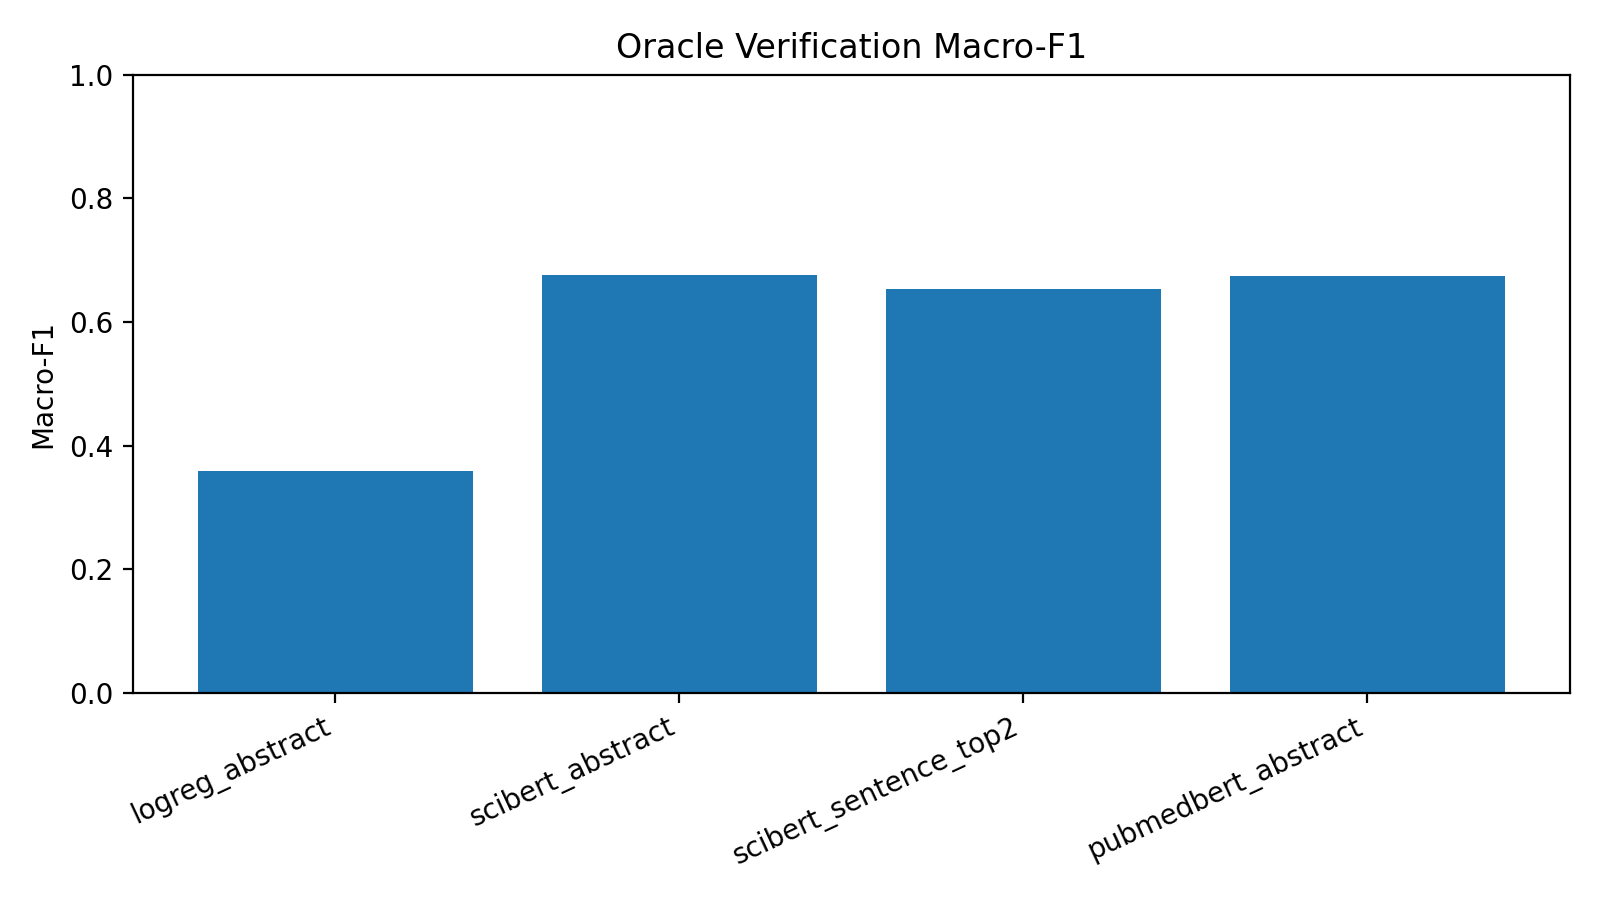
\includegraphics[width=\linewidth]{final_figures/oracle_macro_f1_comparison.png}
\end{minipage}
\hfill
\begin{minipage}{0.48\linewidth}
\centering
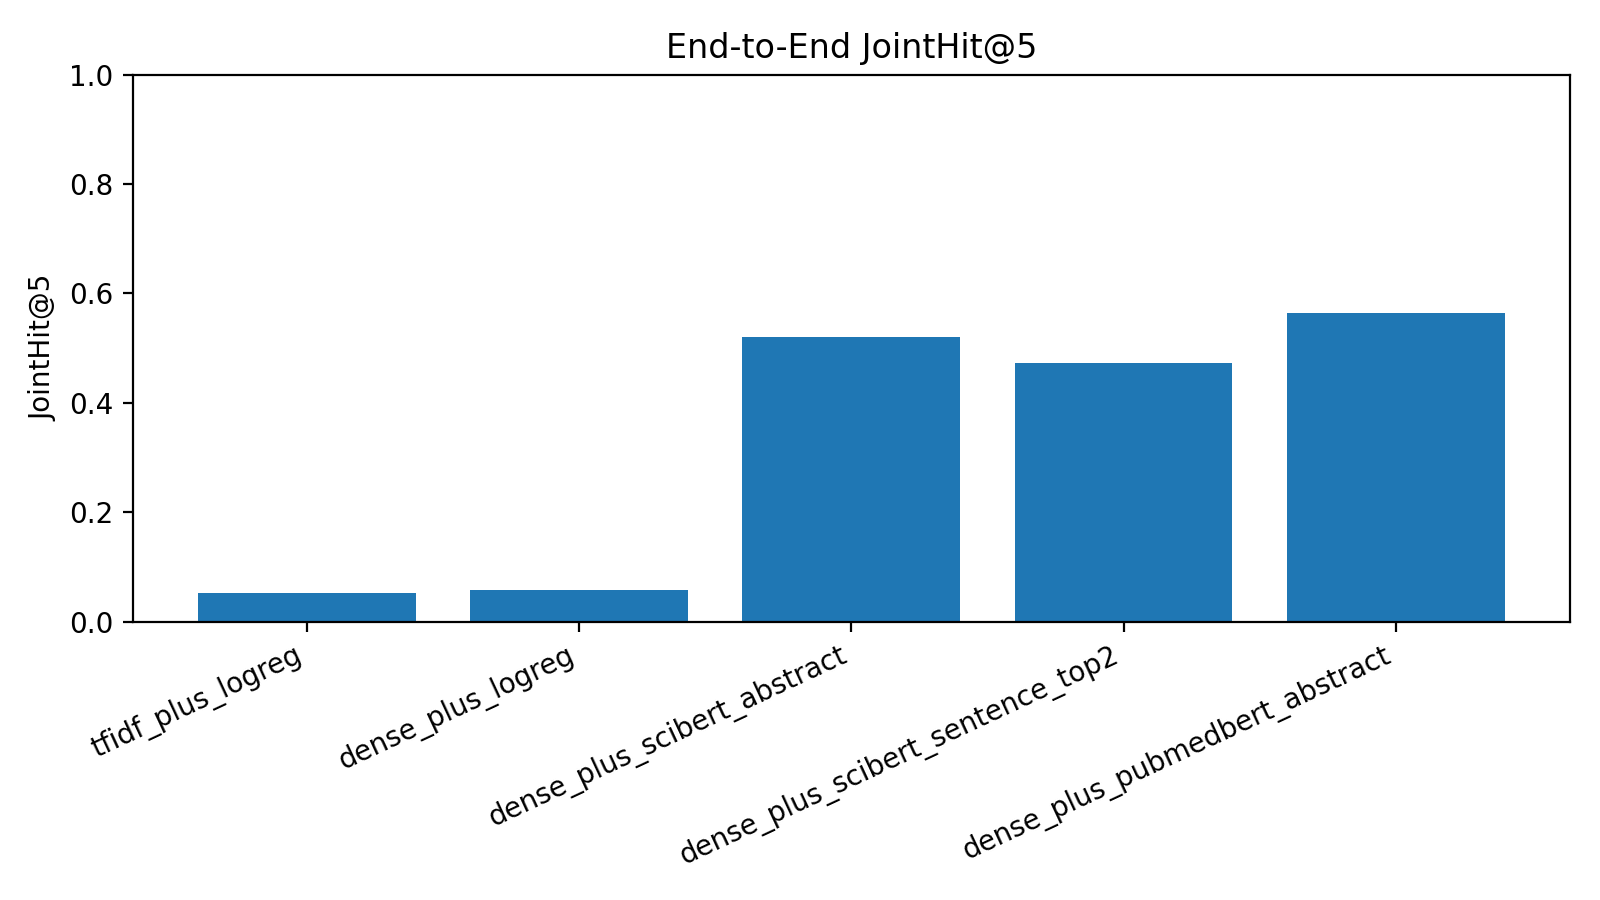
\includegraphics[width=\linewidth]{final_figures/dense_pipeline_joint_hit5_comparison.png}
\end{minipage}
\caption{Left: oracle verifier macro-F1. Right: end-to-end JointHit@5 for dense-retrieval pipelines.}
\label{fig:final_comparison}
\end{figure}

\subsection{Sentence Selection and Error Analysis}
The sentence selector finds relevant rationale sentences reasonably often: Hit@1 is 0.474, Hit@2 is 0.651, and Hit@3 is 0.790 (Table~\ref{tab:analysis}). However, using only the top two selected sentences as verifier input hurts full-pipeline performance, reducing JointHit@5 from 0.521 for Dense+\textsc{SciBERT} with full abstracts to 0.473. This is a useful negative result. The selected sentences often include relevant keywords, but the verifier appears to benefit from broader abstract-level context, especially for distinguishing \textsc{NoInfo} from weak evidence.

The error analysis supports the same interpretation. For Dense+\textsc{SciBERT} at top-5, 98 of 188 evidence-bearing development claims are solved, 24 are retrieval misses, and 66 are stance errors. Thus only 12.8\% of evidence-bearing claims fail because no gold abstract is retrieved in the top five, while 35.1\% fail even though a gold abstract is retrieved. By label, top-5 stance errors are common for both \textsc{Supports} and \textsc{Refutes}: 34 \textsc{Supports} claims and 32 \textsc{Refutes} claims fall into this category. This suggests that remaining progress will depend more on evidence-aware verification than on simply retrieving more abstracts.

\begin{table}[t]
\centering
\small
\begin{tabular}{lccc}
\hline
\textbf{Analysis} & \textbf{Metric 1} & \textbf{Metric 2} & \textbf{Metric 3} \\
\hline
Rationale selection & Hit@1 0.474 & Hit@2 0.651 & Cov.@2 0.502 \\
Top-5 pipeline status & Success 52.1\% & Retrieval miss 12.8\% & Stance error 35.1\% \\
\hline
\end{tabular}
\caption{Final-stage evidence-selection and error-analysis results.}
\label{tab:analysis}
\end{table}

\section{Discussion}
The experiments give a clear picture of the pipeline. First, dense retrieval is better than TF--IDF retrieval, but retrieval alone does not solve the task. Dense retrieval raises evidence recall, yet the logistic-regression verifier remains too weak to use those candidates effectively. Second, domain-specific transformer verifiers are the main source of improvement. \textsc{SciBERT} and \textsc{PubMedBERT} both dramatically outperform the lexical verifier, and \textsc{PubMedBERT} gives the strongest end-to-end system. Third, sentence-level evidence selection is not automatically beneficial. Although the TF--IDF selector often finds gold rationale sentences, compressing the evidence to two sentences removes context that the verifier needs for stance prediction.

The most important takeaway is that the remaining bottleneck is stance verification under realistic retrieval noise. At top-10, dense retrieval misses only 6.9\% of evidence-bearing claims, but the pipeline still fails many claims because the verifier assigns the wrong label to retrieved evidence. Future improvements should therefore focus on better evidence aggregation, rationale-aware training, and calibration between \textsc{NoInfo} and true support/refutation.

\section{Conclusion}
We built and evaluated a retrieval-based scientific claim verification system for SciFact. Dense MPNet retrieval improves evidence retrieval over TF--IDF, and transformer verifiers greatly outperform a lexical classifier. The best final system combines dense retrieval with \textsc{PubMedBERT}, reaching JointHit@5 of 0.564 on the SciFact development set. Error analysis shows that retrieval is reasonably strong and that stance prediction is now the main bottleneck. Our sentence-selection experiment further shows that evidence targeting must preserve enough context for verification, rather than simply shortening abstracts to the most lexically similar sentences.

\section*{Author Contributions}
Jiapei Liao contributed to system implementation, experiment execution, analysis, and report writing. Yuxiang Liu contributed to project design, experiment planning, result interpretation, and report editing.

\begin{thebibliography}{9}

\bibitem[Beltagy et~al.(2019)Beltagy, Lo, and Cohan]{beltagy2019scibert}
Iz Beltagy, Kyle Lo, and Arman Cohan. 2019.
\newblock {SciBERT}: A pretrained language model for scientific text.
\newblock In \textit{Proceedings of the 2019 Conference on Empirical Methods in Natural Language Processing and the 9th International Joint Conference on Natural Language Processing (EMNLP-IJCNLP)}, pages 3615--3620.

\bibitem[Gu et~al.(2021)Gu, Tinn, Cheng, Lucas, Usuyama, Liu, Naumann, Gao, and Poon]{gu2021domain}
Yu Gu, Robert Tinn, Hao Cheng, Michael Lucas, Naoto Usuyama, Xiaodong Liu, Tristan Naumann, Jianfeng Gao, and Hoifung Poon. 2021.
\newblock Domain-specific language model pretraining for biomedical natural language processing.
\newblock \textit{ACM Transactions on Computing for Healthcare}, 3(1):1--23.

\bibitem[Reimers and Gurevych(2019)]{reimers2019sentence}
Nils Reimers and Iryna Gurevych. 2019.
\newblock Sentence-BERT: Sentence embeddings using siamese {BERT}-networks.
\newblock In \textit{Proceedings of the 2019 Conference on Empirical Methods in Natural Language Processing and the 9th International Joint Conference on Natural Language Processing (EMNLP-IJCNLP)}, pages 3982--3992.

\bibitem[Song et~al.(2020)Song, Tan, Qin, Lu, and Liu]{song2020mpnet}
Kaitao Song, Xu Tan, Tao Qin, Jianfeng Lu, and Tie-Yan Liu. 2020.
\newblock MPNet: Masked and permuted pre-training for language understanding.
\newblock In \textit{Advances in Neural Information Processing Systems}, pages 16857--16867.

\bibitem[Wadden et~al.(2020)Wadden, Lin, Lo, Wang, van Zuylen, Cohan, and Hajishirzi]{wadden2020fact}
David Wadden, Shanchuan Lin, Kyle Lo, Lucy Lu Wang, Madeleine van Zuylen, Arman Cohan, and Hannaneh Hajishirzi. 2020.
\newblock Fact or fiction: Verifying scientific claims.
\newblock In \textit{Proceedings of the 2020 Conference on Empirical Methods in Natural Language Processing (EMNLP)}, pages 7534--7550.

\end{thebibliography}

\end{document}
